\section{Overview of signal systematic uncertainties}

Although the data-driven background systematics drive the sensitivity of the analysis, we characterize our signals with simulated data, so these samples have additional NPs which account for the known mismodellings of the simulation compared to the data derived in dedicated control regions
Except for the \et SFs (which were described in detail in \Sect{\ref{subsec:trig-sf-et}}), all these are not custom to the analysis strategy, but follow a dedicated prescription from the collaboration. As such, and because they don't drive our analysis sensitivity, we will just give a very brief summary of them here.

\noindent
\textbf{Detector modelling uncertainties}

To account for the difference in the tagging probability in data, the dedicated FTAG SFs for the \Pqb, \Pqc, and light-jets are applied using the variations measured by the calibrations (described in \Sect{\ref{d1r-calibration}}).
The variation on the jets' energy scale and resolution (JES and JER) are applied, as well as the uncertainty due to the pile-up veto JVT tagger.
We apply an uncertainty for the pile-up reweighting factors that are applied to correct the simulation to the pile-up distribution in data.
Trigger uncertainties from the HLT \Pqb-tag are prescribed by the $b$-jet trigger group and the dedicated \et SFs derived for this analysis are also applied. \hl{How is the uncertainty on ET calculated?}
The uncertainty on the integrated luminosity is a 1.7\% uncertainty on the signal normalization.% Measured with the LUCID-2 detector

\noindent
\textbf{Theoretical Uncertainties}

Differences between the parton shower (PS) and underlying event (UE) are assessed using the differences between the nominal Pythia 8 sample (which uses the Lund string model for the PS) and an alternative Herwig 7 sample (which uses the cluster hadronization model for the PS)
This uncertainty is the largest in the analysis, showing up as an up to 10\% impact on the ggF and VBF acceptances for the.
The $\pm 1 \sigma$ variation templates are derived exclusively for each category, but constrained with a single NP. 

The uncertainty in the matrix element is assessed by varying the renormalization and factorization scales ($\mu_R$ and $\mu_F$) up and down by a factor of 2.
The size of this uncertainty is $\approx$ a 2\% difference on the signals, although it gets as large as 6\% in some analysis categories.
The uncertainties due to the pdfs of the colliding partons are calculated from the $1\sigma$ error bar on the pdf replicas.

For the limits on the SM signal strength, we also include the 3.5\% normalization uncertainty on the  $H\rightarrow b\bar{b}$ branching ratio, and the uncertainties on the theoretical cross-section due to the pdf, $\alpha_s$, renormalization scheme, and $m_t$ scale are accounted for.

%\textbf{I'm confused, does this mean we're double counting some of these uncertainties in the xsec and shape dependence of the samples?}
% I don't think so b/c one is the differential distributions and the other is the signal strength

\begin{table}
\begin{tabular}{c c c}
\toprule
Systematic identifier & Description  & \# of NPs \\
\midrule
{}   & ggF: CR1 / CR2 Shape variations & 3 years x 4 SR quadrants  = 12  \\
{}   & VBF: CR1 / CR2 Shape variations &  4 SR quadrants  = 12  \\
\fcolorbox{soulyellow}{soulyellow}{Background} & 3b1f unc (ggF only) & 3 years  \\
{} & Bootstrap & \# of histogram bins  \\
\hline
{} &  \Pqb-jet  & 3 eigenvariations and 1 extrapolation \\
\fcolorbox{soulpink}{soulpink}{FTAG} & \Pqc-jet eigendecomp &  4 eigenvariations and 1 extrapolation \\
{} & light-jet eigendecomp & 4 eigenvariations \\
\hline
{} & JES & 30 \\
\fcolorbox{soulpurple}{soulpurple}{JET} & JER & 13 \\
{} & JVT & 1 \\
\hline
{}  & pile-up reweighting & 1 \\
\fcolorbox{soulblue}{soulblue}{Data taking} & Luminosity & 1 \\
{} & {HLT + L1 trigger SFs} & 2 \\
\hline
{} & PS, pdf, and scale uncertainties & 3 x 2 (ggF + VBF) ) = 6  \\
\fcolorbox{soulgreen}{soulgreen}{Theory} & BR $H \rightarrow b\bar{b}$ (*) & 1  \\
{} & Cross-section uncertainties (*) & 4 \\
\bottomrule
\end{tabular}
\caption{Note: the (*) indicates these are not included in the \kl and \k2v scans.}
\end{table}


\subsection{S+B fits}

From a background-only fit and signal + background fits, the NP pulls are shown in \Fig{\ref{fig:ggf_vbf-pulls-corr-bonly}}.

\noindent
\begin{figure}
\begin{minipage}{0.48\textwidth}
\centering
\fcolorbox{soulyellow}{soulyellow}{Background}
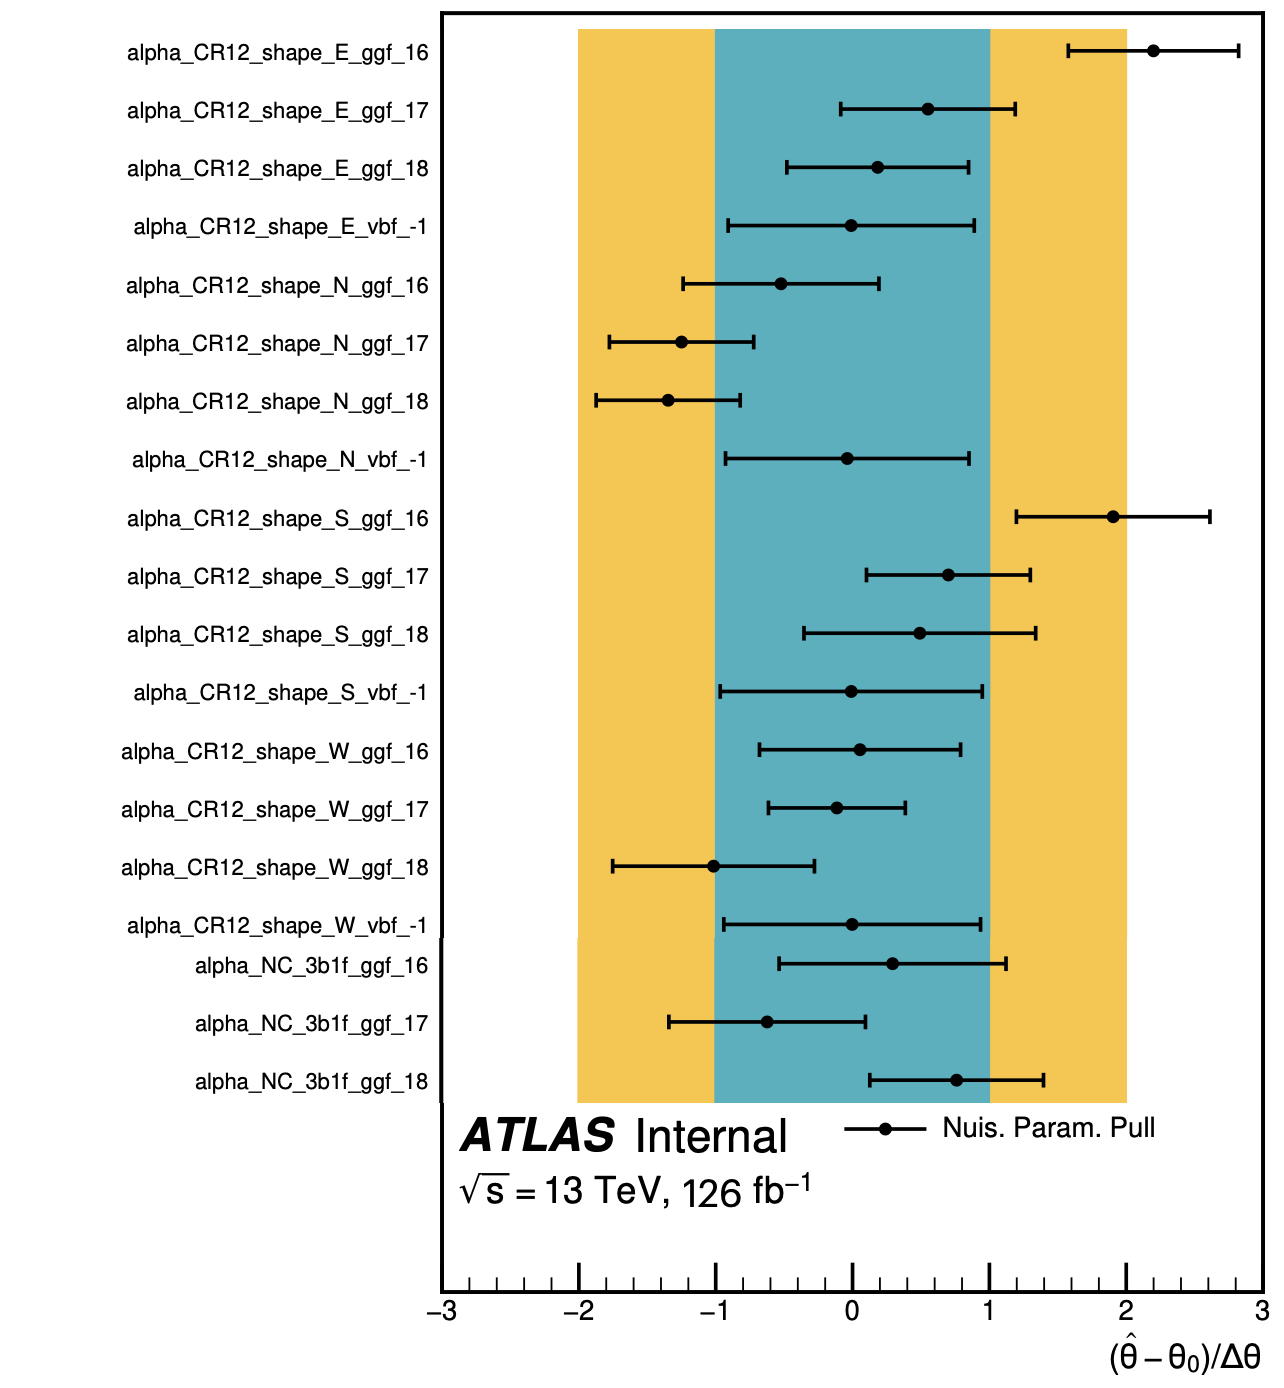
\includegraphics[width=.9\textwidth]{figures/my_dihiggs/BKG-bkg-only-pulls} 
\\
\vspace{.75em}
\fcolorbox{soulblue}{soulblue}{Data taking} 
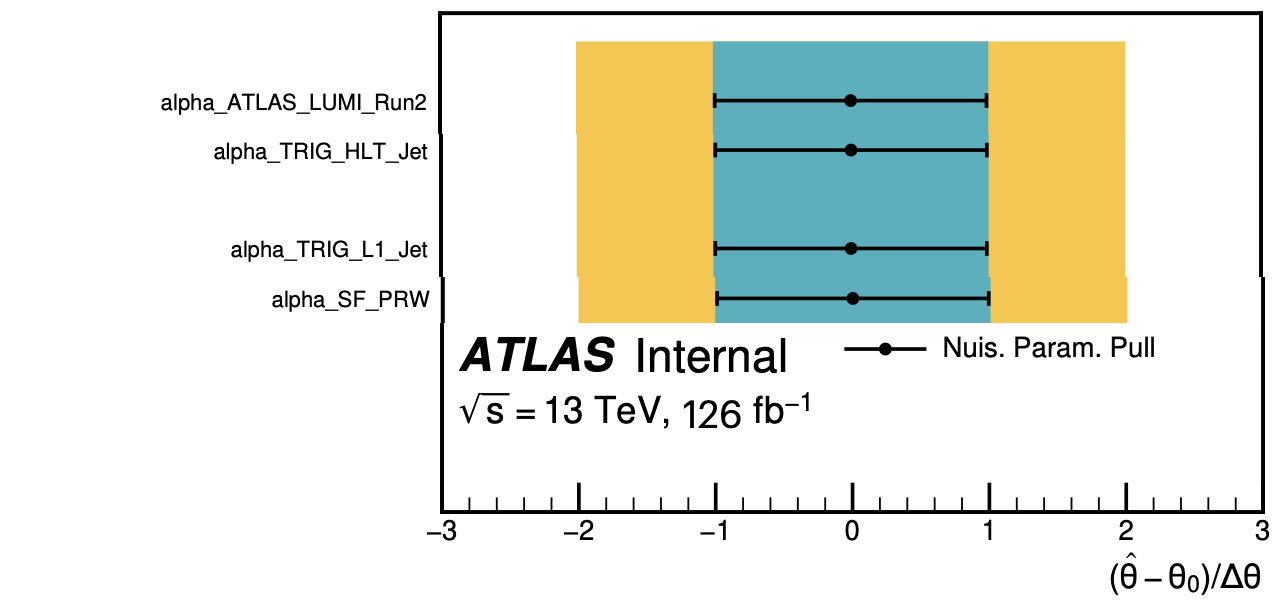
\includegraphics[width=.85\textwidth]{figures/my_dihiggs/DATA-bkg-only-pulls}
\\
\vspace{.75em}
\fcolorbox{soulgreen}{soulgreen}{Theory}
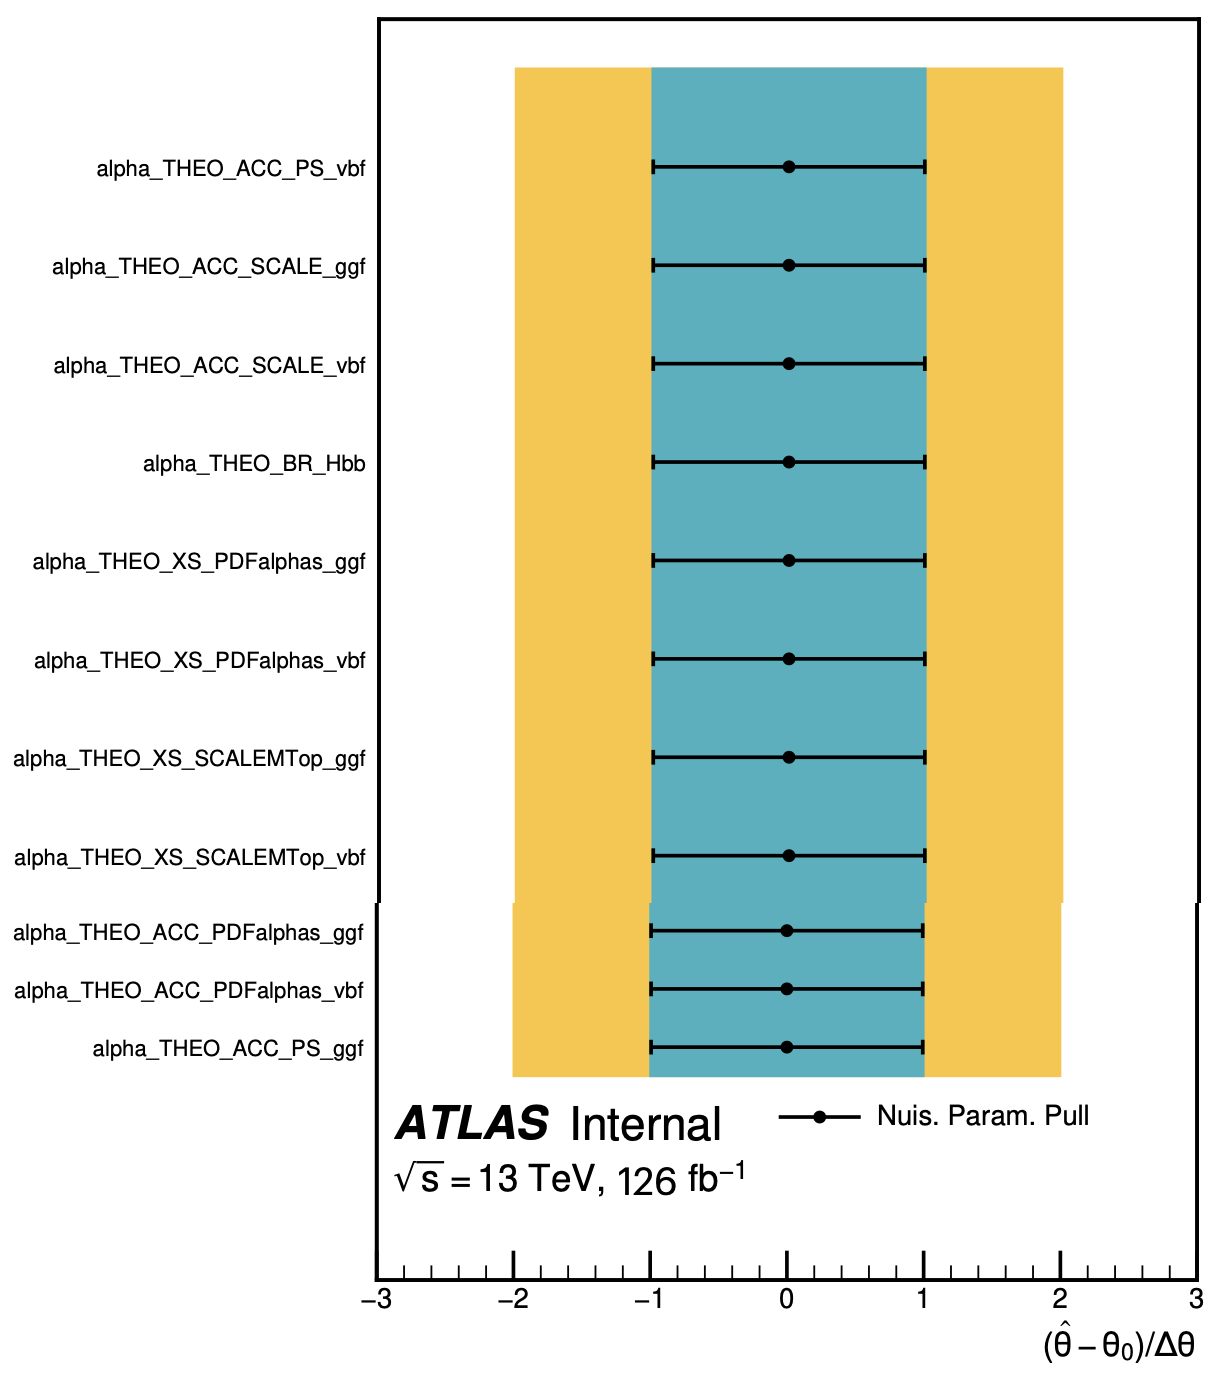
\includegraphics[width=.88\textwidth]{figures/my_dihiggs/THEO-bkg-only-pulls}
\end{minipage}
%
\begin{minipage}{0.5\textwidth}
\centering
\fcolorbox{soulpink}{soulpink}{FTAG} 
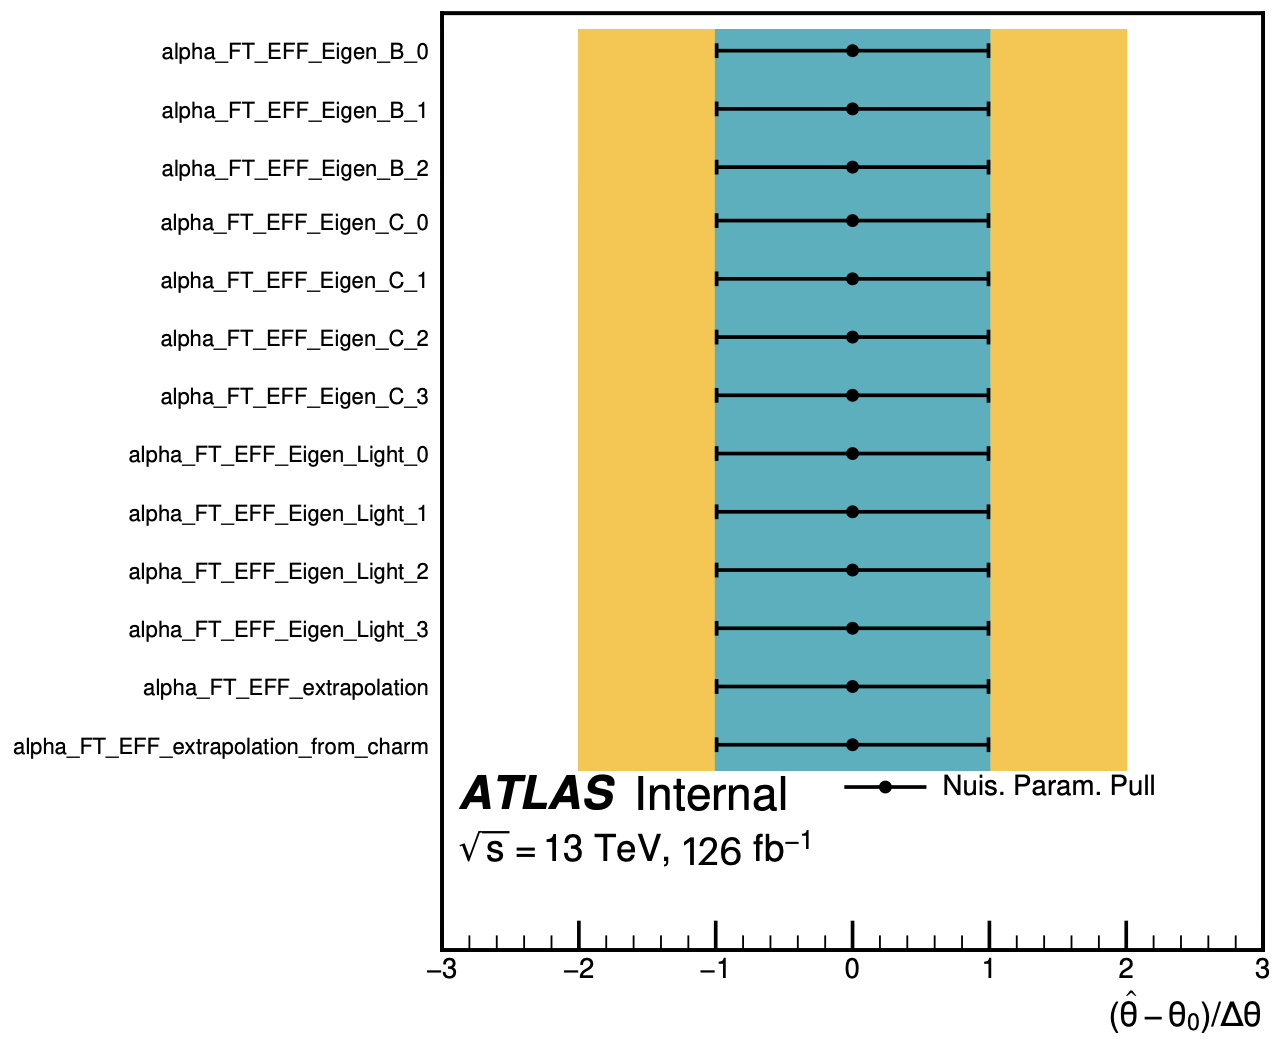
\includegraphics[width=.9\textwidth]{figures/my_dihiggs/FTAG-bkg-only-pulls}
\\
\fcolorbox{soulpurple}{soulpurple}{JET} 
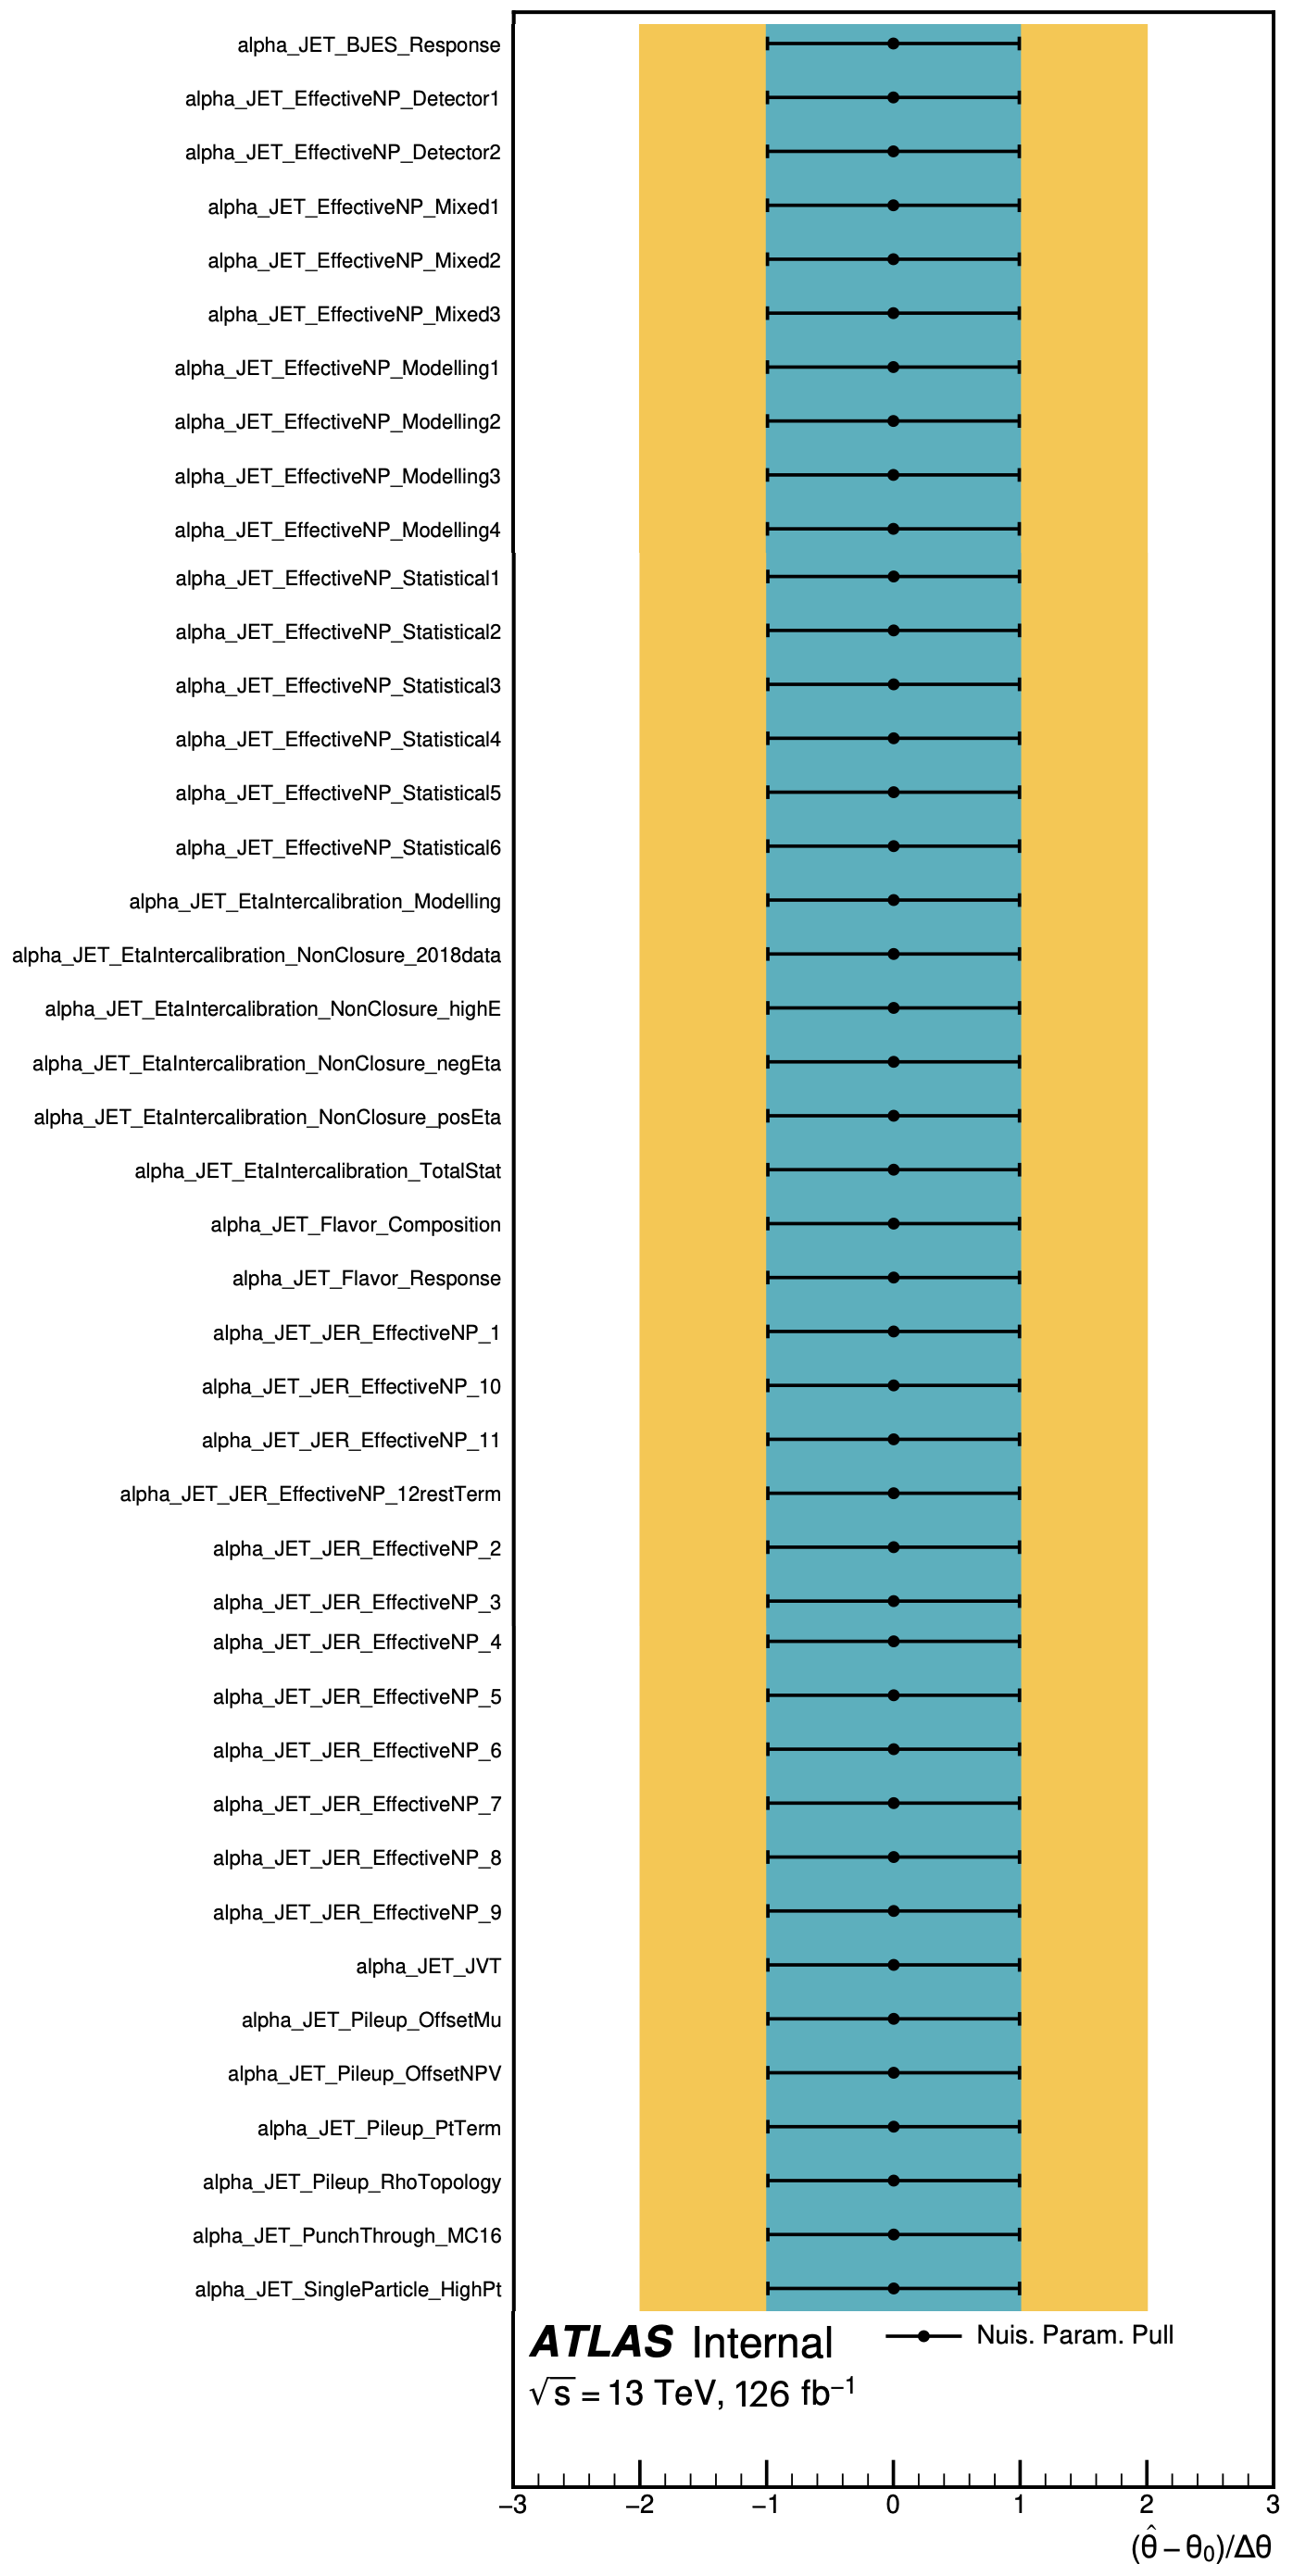
\includegraphics[width=.9\textwidth]{figures/my_dihiggs/JET-bkg-only-pulls}	
\end{minipage}
\caption{Pulls for the fit to the background template.}
\label{fig:ggf_vbf-pulls-corr-bonly}
\end{figure}

